\documentclass[xcolor={usenames,svgnames,x11names,dvipsnames,table}]{beamer}

\usetheme{SBUclass}

\usepackage{mypackages}
\usepackage{mycommands}

\title{\texorpdfstring{Language \& Technology}{Language and Technology}}
\subtitle{Wrapping Up}
\author{Thomas Graf}
\institute{Stony Brook University\\\texttt{lin120@thomasgraf.net}}
\date{}


\begin{document}
\unnumbered{
\begin{frame}
	\titlepage
\end{frame}
}

\begin{frame}{Be Skeptical}
    \begin{itemize}
        \item Humans overestimate technology.\\
            \subpoint{Loebner Prize\slash Turing test}
        \item Don't buy the hype.\\
            \subpoint{deep learning, artificial intelligence, culturomics, neuroscientism, \ldots}
        \item Technological advances also come with downsides.\\
            \subpoint{unemployment, rising job requirements, mass surveillance, \ldots}
    \end{itemize}
\end{frame}

\begin{frame}{The State-of-the-Art in Language Technology} 
    \begin{itemize}
        \item Almost everything involves \highlight{n-grams models}.
            %
            \begin{itemize}
                \item word completion\slash prediction
                \item stylistic analysis
                \item OCR
                \item spell checking
                \item web search
                \item word meaning
                \item machine translation
            \end{itemize}
        \item Frequency information from corpora\slash tree banks is used to\\
            add \highlight{probabilities} to the models.
    \end{itemize}
\end{frame}

\begin{frame}{Language is Complex}
    \begin{itemize}
        \item Language comes easy to humans,\\
            but it is \highlight{incredibly complex}.
            \begin{itemize}
                \item culture-specific rules of turn taking
                \item hidden structure of sentences
                \item how that hidden structure is inferred
                \item building sentence meaning from word meaning
                \item tons of variation across languages and dialects
            \end{itemize}
        \item We have to deal with this complexity.
        \item Probabilities won't cut it because of \highlight{Zipf's law}.
    \end{itemize}
\end{frame}

\begin{frame}{Related Linguistics Courses}
    \begin{itemize}
        \item LIN 101 \emph{Human Language}\\
        \item LIN 110 \emph{Anatomy of English Words}\\
        \item LIN 200 \emph{Language in the USA}\\
        \item as background for sentence models:\\
            LIN 311 \emph{Syntax}\\
            LIN 346 \emph{Language \& Meaning}\\
        \item as background for speech recognition:\\
            LIN 201 \emph{Phonetics}\\
            LIN 301 \emph{Phonology}
    \end{itemize}

    \pause
    \begin{block}{Planned Course for Fall 2018}
        \begin{itemize}
            \item LIN 425 \emph{Computational Data Analysis}
            \item computer-assisted statistics and data analysis
            \item useful for both computational and experimental linguistics
        \end{itemize}
    \end{block}
\end{frame}

\begin{frame}{My Computational Courses This Coming Spring}
    \begin{enumerate}
        \item \textbf{LIN 488 Internship}\\
            Help me adapt my Jupyter notebooks on mathematics in linguistics for an undergraduate audience.
        \item \textbf{LIN 630 Parsing \& Processing}\\
            Computational parsing techniques and how they compare to human sentence processing.\\
            \emph{Prerequisite}: LIN 311 Syntax
    \end{enumerate}
\end{frame}

\begin{frame}{Two Course Recommendations Outside Linguistics}
    \begin{enumerate}
        \item SOC 330 \emph{Media and Society}\\
            (Jason J.~Jones; no programming, but a bit of computational sociology and big data)
        \item AMS 103 \emph{Applied Math in Technology}\\
            (Matthew Reuter; includes a live cookie baking session)
    \end{enumerate}
\end{frame}

\begin{frame}{Programming Concepts}
    \begin{itemize}
        \item \textbf{Universal}
            \begin{itemize}
                \item strings, integers, lists
                \item variables
                \item print, input
                \item conditionals
                \item while loops
                \item for loops
                \item custom functions
                \item regular expressions
            \end{itemize}
        \item \textbf{Python-Specific}
            \begin{itemize}
                \item counters
                \item positions and slices
                \item built-in functions like \texttt{len}, \texttt{str.lower}, \ldots
            \end{itemize}
    \end{itemize}
\end{frame}

\begin{frame}{Sticking with Python}
    \begin{itemize}
        \item You invested lots of time and energy on picking up some programming skills.
              They \highlight{should not go to waste}!
        \item The most important thing: find yourself a \highlight{project}!
    \end{itemize}

    \begin{block}{Project suggestions}
        \begin{itemize}
            \item Computational analysis in a book report
            \item Automatic menu generator for New York hipster restaurants
            \item Facebook bot to like all your friends' posts and\\
                  leave a short reply
            \item Script to delete all unread emails that are older than 30 days
            \item Reminder to take a break after 2h in front of the screen
            \item Automating something you frequently do manually
        \end{itemize}
    \end{block}
\end{frame}

\begin{frame}{Some Project Ideas from Reddit}
    Check out the \href{https://www.reddit.com/r/Python/comments/308ucq/how_do_you_use_python_to_automate_tasks_in_life/}{Reddit thread}:

    \medskip
    \pause
    \begin{quote}
        Our department keeps a calendar of activities in excel.
        I use python to import that spreadsheet, break the activities into itemized tasks, put due dates on each task, and spit out those tasks for each teammate.
    \end{quote}

    \pause
    \begin{quote}
        I stitched together a video encoding script, a mp3 tag reading script and a YouTube uploading script to automatically upload all of the old music I'd recorded to YouTube. Saved me 100s of hours of manual work. 
    \end{quote}
\end{frame}

\begin{frame}{Some Project Ideas from Reddit [cont.]}
    \begin{quote}
        This is a pretty silly usage, but the autopy package is really great for making auto-clickers for various web-games. 
    \end{quote}

    \pause
    \begin{quote}
        I have a script that checks the Powerball and Megamillions jackpot size and calculates the expectation value of a play. If either is positive, it sends me a text to buy a ticket.
    \end{quote}

    \pause
    \begin{quote}
        Not complete yet, but I am using python on a RasPi to automate the temperature, humidity, and lighting for my two pythons' cages
    \end{quote}
\end{frame}

\begin{frame}{Some Project Ideas from Reddit [cont.]}
    \begin{quote}
        My brother in law has a "habit" of going to jail.
        All. The. Time.
        My wife wants to know when it happens, so I setup a script to poll the local jail inmate rosters, and send me an email when his name shows up.
        It works pretty well.
    \end{quote}
\end{frame}

\begin{frame}{Other Fun Stuff with Python}
    \begin{itemize}
        \item Python coding for \emph{Minecraft}\\
            \href{http://www.instructables.com/id/Python-coding-for-Minecraft/}{http://www.instructables.com/id/Python-coding-for-Minecraft/}
        \item Modding \emph{The Sims 4}\\
            \href{http://simswiki.info/wiki.php?title=Tutorials:TS4_General_Modding}{http://simswiki.info/wiki.php?title=Tutorials:TS4\_General\_Modding}
        \item Creating hi-res texture mods (e.g.\ for Resident Evil 4 HD)\\
            \href{https://youtu.be/u_8I3vaVrfE}{https://youtu.be/u\_8I3vaVrfE}
        \item \emph{Gray Hat Python} book on hacking with Python
    \end{itemize}
\end{frame}

\begin{frame}{Code Combat \& Code Wars}
    \centering

    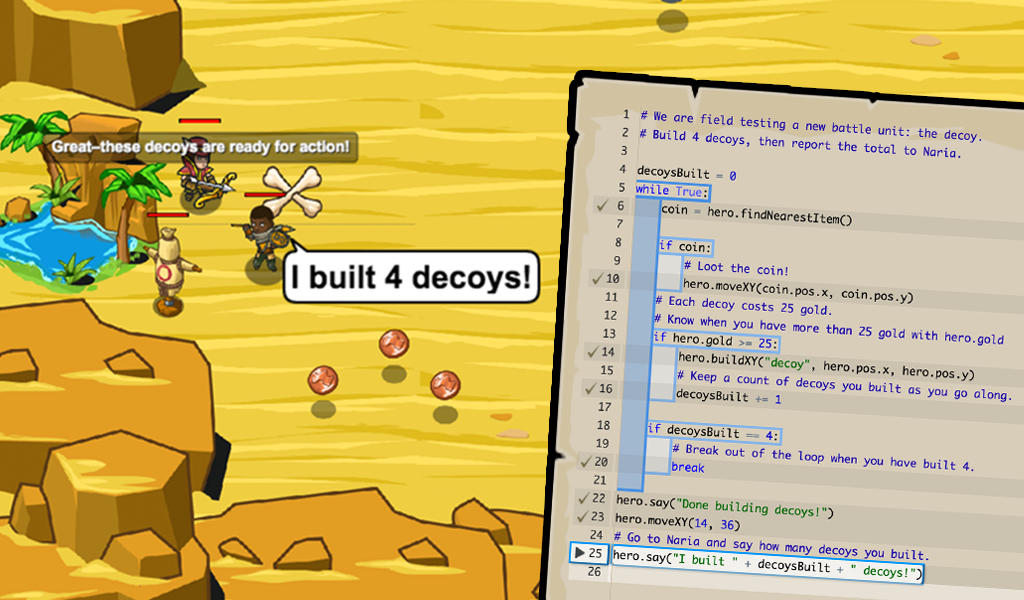
\includegraphics[width=.8\linewidth]{./img/codecombat}

    If you liked Code Combat, check out \href{https://www.codewars.com/}{Code Wars}!
\end{frame}

\begin{frame}{How much Python Do I Know?}
    \begin{itemize}
        \item We covered enough Python for 90\% of all problems.
        \item But Python can do a lot more:
            \begin{itemize}
                \item strides
                \item dictionaries (of which Counters are a special case)
                \item unpacking
                \item zipping
                \item recursive functions
                \item object oriented programming with classes
                \item generators
                \item decorators
            \end{itemize}
        \item And there's many powerful libraries:
            \begin{itemize}
                \item pyplot
                \item pandas
                \item ntlk
                \item scipy
                \item scikit-learn
            \end{itemize}
        \item Don't worry about any of this for now.
    \end{itemize}
\end{frame}

\begin{frame}{Additional Teaching Materials}
    If at some point you need to know more Python for your project,
    check out some of these:

    \begin{itemize}
        \item The remainder of our textbook\\
                \emph{Automate the Boring Stuff With Python}
        \item The programming historian\\
            \href{http://programminghistorian.org/}{http://programminghistorian.org/}
        \item Python programming for the humanities\\
            \href{http://www.karsdorp.io/python-course/}{http://www.karsdorp.io/python-course/}
        \item Natural language processing with Python\\
            \href{http://www.nltk.org/book/}{http://www.nltk.org/book/}
        \item Mark Summerfield's book \emph{Programming in Python 3}
        \item For more theory, check out the book \emph{Language and Computers}
    \end{itemize}
\end{frame}

\begin{frame}{Don't do it Alone!}
    \begin{itemize}
        \item Form learning\slash reading groups with your classmates.
        \item Check out SBU undergraduate clubs and the events they host.
        \item Join online communities.
        \item Need advice?
            Send me an email or come to my office hours!
    \end{itemize}
\end{frame}

\begin{frame}{The Future}
    \begin{itemize}
        \item We have launched an M.A. in Computational Linguistics. 
        \item And we are developing a B.A., too.
        \item So expect more UG CompLing courses in the future!
        \item \textbf{CompLing Info Session:} Wednesday, December 13
    \end{itemize}

    \begin{block}{Additional Announcements}
        I will post one or two items to Blackboard this month\\
        that might be of interest to you.
    \end{block}
\end{frame}

\end{document}
